\documentclass[11pt,a4paper]{article}
\usepackage[utf8]{inputenc}
\usepackage{color}
\usepackage{enumerate}
\usepackage{fancyhdr}
\usepackage{minted}
\usepackage{graphicx}
\usepackage{array}
\usepackage{hyperref}
\usepackage{amssymb,amsmath}
\usepackage{multirow}
\usepackage[spanish, es-tabla]{babel}
\usepackage[math]{iwona}
\usepackage{titlesec}
\usepackage{varwidth}

\setlength{\oddsidemargin}{18pt}
\setlength{\headheight}{14pt}
\setlength{\textheight}{672pt}
\setlength{\marginparsep}{11pt}
\setlength{\footskip}{30pt}
\hoffset = 0pt
\voffset = 0pt
\setlength{\topmargin}{0pt}
\setlength{\headsep}{25pt}
\setlength{\textwidth}{424pt}
\setlength{\marginparwidth}{54pt}
\setlength{\marginparpush}{5pt}
\paperwidth = 597pt
\paperheight = 845pt

\pagestyle{fancy}
\fancyhead[LO]{\textcolor[rgb]{0,0,0}{Grado en Ingeniería Informática}}
\fancyhead[RO]{\textcolor[rgb]{0.2,0.2,0.9}{Visión por Computador, Curso 2017-2018}}

\hypersetup{
    colorlinks,
    citecolor=black,
    filecolor=black,
    linkcolor=black,
    urlcolor=blue
}

\newcommand{\horrule}[1]{\rule{\linewidth}{#1}}

\newmintedfile[PasoUno]{python}{
    firstline=26,
    lastline=47,
    numbersep=5pt,
    gobble=0,
    frame=lines,
    framesep=2mm,
    tabsize=3,
}

\newmintedfile[PasoDos]{python}{
    firstline=51,
    lastline=67,
    numbersep=5pt,
    gobble=0,
    frame=lines,
    framesep=2mm,
    tabsize=3,
}

\newmintedfile[PasoTres]{python}{
    firstline=69,
    lastline=86,
    numbersep=5pt,
    gobble=0,
    frame=lines,
    framesep=2mm,
    tabsize=3,
}

\newmintedfile[PasoCuatroNormaUno]{python}{
    firstline=11,
    lastline=13,
    numbersep=5pt,
    gobble=0,
    frame=lines,
    framesep=2mm,
    tabsize=3,
}

\newmintedfile[PasoCuatroNormaDos]{python}{
    firstline=15,
    lastline=17,
    numbersep=5pt,
    gobble=0,
    frame=lines,
    framesep=2mm,
    tabsize=3,
}

\newmintedfile[PasoCuatroNormaDosHys]{python}{
    firstline=19,
    lastline=22,
    numbersep=5pt,
    gobble=0,
    frame=lines,
    framesep=2mm,
    tabsize=3,
}

\newmintedfile[PasoCuatro]{python}{
    firstline=90,
    lastline=97,
    numbersep=5pt,
    gobble=0,
    frame=lines,
    framesep=2mm,
    tabsize=3,
}

\newmintedfile[ExtraerNegativos]{python}{
    firstline=138,
    lastline=144,
    numbersep=5pt,
    gobble=0,
    frame=lines,
    framesep=2mm,
    tabsize=3,
}

\newmintedfile[ExtraerCaracteristicas]{python}{
    firstline=99,
    lastline=135,
    numbersep=5pt,
    gobble=0,
    frame=lines,
    framesep=2mm,
    tabsize=3,
}

\newmintedfile[EscaneoSimple]{python}{
    firstline=257,
    lastline=288,
    numbersep=5pt,
    gobble=0,
    frame=lines,
    framesep=2mm,
    tabsize=3,
}

\newmintedfile[NMS]{python}{
    firstline=208,
    lastline=238,
    numbersep=5pt,
    gobble=0,
    frame=lines,
    framesep=2mm,
    tabsize=3,
}

\newmintedfile[EscaneoNMS]{python}{
    firstline=290,
    lastline=322,
    numbersep=5pt,
    gobble=0,
    frame=lines,
    framesep=2mm,
    tabsize=3,
}

\newmintedfile[EntrenamientoClasificadores]{python}{
    firstline=246,
    lastline=255,
    numbersep=5pt,
    gobble=0,
    frame=lines,
    framesep=2mm,
    tabsize=3,
}

\newmintedfile[ClasificadorVotos]{python}{
    firstline=240,
    lastline=244,
    numbersep=5pt,
    gobble=0,
    frame=lines,
    framesep=2mm,
    tabsize=3,
}

\newmintedfile[EscaneoVotos]{python}{
    firstline=324,
    lastline=356,
    numbersep=5pt,
    gobble=0,
    frame=lines,
    framesep=2mm,
    tabsize=3,
}

\begin{document}

    \begin{titlepage}

        \centering

        \begin{figure}[h]

            \centering
            
\includegraphics[width=0.6\textwidth]{logo-ugr.png}

        \end{figure}

        \vspace{1cm}

        {\scshape\LARGE Universidad de Granada}

        \vspace{1cm}

        {\LARGE Visión por Computador}

        \vspace{1cm}

        \horrule{0.5pt} \\[0.4cm]

        {\huge\bfseries\textit{Proyecto final}} \\

        \horrule{2pt} \\[0.5cm]

        \vspace{1cm}

        {\itshape\large Laura Calle Caraballo \\
        Javier León Palomares}

        \vfill

        {\Large\today}

    \end{titlepage}

\newpage

    \tableofcontents
    \listoffigures

\newpage

    \section{Introducción}

        \par
        El objetivo de este proyecto es explorar la técnica de \textbf{Histograma de Gradientes} (\textit{HoG}) aplicada a la detección de peatones, descrita en \textit{Histograms of Oriented Gradientes for Human Detection} (2005) de \textit{Dalal} y \textit{Triggs}.

        \par
        Para ello, hemos implementado distintos aspectos del método realizando una serie de decisiones de diseño y hemos utilizado la base de datos original para comparar resultados. Las herramientas empleadas son \textit{Python} y las librerías \texttt{OpenCV}, \texttt{NumPy} y \texttt{scikit-learn}.

    \section{Descripción de la técnica e implementación}

        \par
        El \textbf{Histograma de Gradientes} nos permitirá extraer características relevantes de una imagen para poder proceder a su clasificación (contiene un peatón o no). Consta de varias etapas que analizaremos a continuación.

        \subsection{Cálculo de gradientes}

            \par
            El primer paso del proceso es calcular los gradientes horizontales y verticales de cada imagen. Para ello, utilizaremos un \textit{kernel} unidimensional $\left[-1,0,1\right]$ centrado en cada píxel a evaluar.

            \par
            Utilizando los valores anteriores obtendremos las orientaciones de los cambios de intensidad y sus magnitudes. Posteriormente, ya que las imágenes son a color, elegiremos el canal con mayor magnitud de gradiente para cada píxel.

            \par
            El código correspondiente a esta parte es:

            \PasoUno[label=.]{../pedestrian_detection.py}

            \par
            Para obtener las orientaciones de los gradientes (limitándolas al rango $[0,180]$) y sus magnitudes hemos usado \texttt{cartToPolar}, que implementa las siguientes fórmulas:

            $$\theta = \arctan{\frac{g_y}{g_x}}$$
            $$g = \sqrt{g_{x}^2 + g_{y}^2}$$

            \par
            Respecto a la selección del canal de color con mayor respuesta para cada píxel, la aproximación más directa sería utilizando dos bucles anidados para recorrer la imagen píxel por píxel, pero es posible ganar ligeramente en eficiencia aprovechando la capacidad de vectorización de \texttt{NumPy}: generamos todas las combinaciones de posiciones de la imagen, siendo cada una representada por \texttt{(coord\_0[i],coord\_1[i])}; obtenemos los índices del canal con mayor respuesta en cada píxel; finalmente, cada posición estará representada junto a su canal elegido por \texttt{(coord\_0[i],coord\_1[i],indices[i])}. De esta forma, podemos aprovechar la indexación por conjuntos de índices para resumir el proceso de selección en una única línea.

        \subsection{Obtención de histogramas}

            \par
            El uso de histogramas locales se basa en que la forma distintiva de un objeto se puede caracterizar muchas veces con suficiente calidad utilizando distribuciones y orientaciones de gradientes por áreas de una imagen. Además, al resumir implícitamente la información, la dimensionalidad del vector de características se reduce.

            \par
            Para calcular estos histogramas, vamos a dividir la imagen en celdas cuadradas de un cierto número de píxeles (en nuestro caso, $8\times8$). En cuanto a los  histogramas, estarán formados por 9 secciones que corresponden a intervalos de 20 grados entre 0 y 180, puesto que tomaremos las orientaciones por dirección y no por sentido. Para conocer la aportación del ángulo en un píxel, haremos una interpolación lineal que reparta su influencia entre las dos secciones más cercanas; por ejemplo, si tenemos un ángulo de 35 grados, aportará el 25\% de su valor de magnitud a la sección centrada en 20 y el 75\% restante a la centrada en 40.

            \PasoDos[label=.]{../pedestrian_detection.py}

            \par
            Como se puede apreciar, hacemos uso de vectorización para calcular en pocas líneas las aportaciones de todos los píxeles de la celda a las secciones del histograma.

            \par
            Cabe mencionar que tanto el tamaño de las celdas como la disposición de los histogramas en 9 categorías cubriendo el rango $\left[0,180\right]$ se han elegido así porque producen resultados de mayor calidad según el artículo. Asimismo, en el caso de las celdas un tamaño de $8\times8$ permite que haya un número exacto de éstas en las ventanas de $64\times128$ píxeles que luego usaremos para detectar peatones.

            \par
            Finalmente, veamos cómo se usa la función a la hora de calcular todos los histogramas de una imagen:

            \PasoTres[label=.]{../pedestrian_detection.py}

            \par
            Lo primero que hacemos es eliminar el borde que pueda tener la imagen hasta que sus dimensiones sean múltiplos del tamaño de celda. Esto se hace principalmente porque los ejemplos positivos de peatones en los conjuntos de entrenamiento y test tienen un tamaño ligeramente mayor al de $64\times128$ que vamos a necesitar.

            \par
            Posteriormente, recorremos la imagen en saltos de 8 píxeles de izquierda a derecha y de arriba abajo para ir obteniendo los histogramas de toda la malla de celdas.

        \subsection{Normalización de histogramas}

            \par
            La alta variabilidad de contextos y grados de iluminación que existe en la realidad provoca que los gradientes que calculamos se muevan en rangos muy amplios. Puesto que esto puede añadir una complejidad significativa a la ya difícil tarea de distinguir entre una clase y todo lo demás, es necesario el uso de normalización para tener una escala unificada de magnitudes entre 0 y 1.

            \par
            En nuestro caso, esta normalización se realiza agrupando las celdas en bloques cuadrados (por defecto, de $2\times2$ celdas) y aplicando el proceso con una cierta superposición entre dichos bloques (por defecto, 50\%). La superposición, aunque pueda introducir redundancia, aporta calidad al proceso y mejora los resultados, guiándonos por las conclusiones de los autores de la técnica.

            \par
            Según el cálculo realizado para normalizar, podemos distinguir entre las tres variantes probadas:

            \begin{itemize}

                \item
                División entre la norma L1:
                \PasoCuatroNormaUno[label=.]{../pedestrian_detection.py}

                \item
                División entre la norma L2:
                \PasoCuatroNormaDos[label=.]{../pedestrian_detection.py}

                \item
                División preliminar entre la norma L2, recorte de valores superiores a 0.2 y división entre su nueva norma L2 (llamada norma L2-Hys en el artículo):
                \PasoCuatroNormaDosHys[label=.]{../pedestrian_detection.py}

            \end{itemize}

            \par
            La forma de aplicar lo anterior se traduce en la siguiente función:

            \PasoCuatro[label=.]{../pedestrian_detection.py}

            \par
            La función recibe como parámetro el conjunto de histogramas, así como la normalización que aplicará, el tamaño de los bloques y el solapamiento entre los mismos. Tras calcular el intervalo entre cada par de bloques, los recorremos y añadimos cada conjunto resultante de histogramas normalizados al vector de características de la imagen.

    \section{Detección de peatones}

        \subsection{Obtención de datos}

            \par
            Para la detección se ha utilizado un tamaño de ventana de $64\times128$ píxeles, cuya forma permite abarcar personas aproximadamente erguidas. Asimismo, dentro de las ventanas con ejemplos positivos de entrenamiento y test, parte de este tamaño es un borde alrededor del peatón que añade contexto útil; los autores comprobaron que reducir este borde causaba una pérdida notable de precisión.

            \par
            Con los ejemplos positivos ya proporcionados, nuestra próxima tarea será conseguir ejemplos negativos del mismo tamaño a partir de las fotografías del conjunto de datos que no contienen personas. Siguiendo el procedimiento original, vamos a extraer 10 ventanas aleatorias de cada una de esas imágenes. Para no tener que generar miles cada vez que queramos entrenar un clasificador, las guardamos una única vez:

            \ExtraerNegativos[label=.]{../pedestrian_detection.py}

            \par
            Una vez tenemos todas las imágenes necesarias, es el momento de aplicar el proceso descrito en el apartado anterior a cada una de ellas para obtener las características con las que trabajarán los clasificadores de peatones. En código esto se traduce en recorrer los directorios de ejemplos positivos y negativos y utilizar las distintas funciones que calculan un \textbf{Histograma de Gradientes}:

            \ExtraerCaracteristicas[label=.]{../pedestrian_detection.py}

            \par
            Por eficiencia, creamos la matriz que contendrá los vectores de características de todos los ejemplos de entrenamiento en lugar de extenderla a cada paso. Esto requiere conocer el tamaño de dichos vectores de antemano, algo que nos podemos permitir si analizamos cómo hacemos el cálculo del \textbf{Histograma de Gradientes}: utilizamos ventanas de $64\times128$ píxeles, celdas de $8\times8$ píxeles y una superposición del 50\% en bloques de $2\times2$ celdas; si en una ventana caben 16 filas de 8 celdas, esto significa que hay 15 filas de 7 bloques cada una; además, cada bloque contiene 4 celdas, que producen histogramas de 9 casillas. Esto produce un total de $15\cdot7\cdot4\cdot9$ características.

            \par
            Tal como se mencionó anteriormente, las imágenes positivas ya incluidas en el conjunto de datos tienen un borde que incrementa un poco el tamaño, por lo que antes de procesar cada una hay que conocer cuánto vale ese borde para que \texttt{computeCellHistograms} trabaje sobre $64\times128$.

            \par
            Llamaremos a esta función dos veces: una para crear los datos de entrenamiento y otra para crear los datos de test.

        \subsection{Selección del método de normalización de gradientes}

            \par
            Como hemos dicho, podemos optar entre tres normalizaciones distintas, por lo que el primer paso es elegir una de ellas para enfocar futuras mejoras. Con este objetivo en mente, vamos a comparar la calidad de las predicciones de test usando un \textit{SVM} preliminar con $C = 1$ (valor por defecto):

            \vspace{0.3cm}

            \begin{table}[H]

				\centering

				\begin{tabular}{| >{\centering\arraybackslash}m{1.2in} | >{\centering\arraybackslash}m{1.2in} |}

					\hline
					\textbf{Normalización} & \textbf{Precisión} \\
					\hline
					Norma L1 & 96.556\% \\
					\hline
					Norma L2 & 98.446\% \\
					\hline
					Norma L2-Hys & 98.093\% \\
					\hline

				\end{tabular}

			\end{table}

            \par
            A la vista de los resultados, elegimos la norma L2 como método de normalización a partir de ahora. En cuanto a los porcentajes de acierto, son aceptables, pero si tenemos en cuenta que en cada imagen real habremos de analizar un gran número de ventanas para encontrar personas, nos interesa tratar de mejorar estas cifras.

        \subsection{Ajustes adicionales del modelo}

            \par
            En esta sección vamos a buscar brevemente alguna forma de incrementar la precisión del modelo, para lo que contemplaremos dos factores: el parámetro C (que controla la penalización de los errores de clasificación) y el hecho de que las clases no están equilibradas (la clase no-peatón tiene muchos más ejemplos porque su variabilidad es mayor). Para el parámetro C vamos a probar el valor de 0.01 que usan los autores, y para el equilibrio de clases vamos a ponderar su peso de forma inversa a su frecuencia.

            \begin{table}[H]

				\centering

				\begin{tabular}{| >{\centering\arraybackslash}m{1.8in} | >{\centering\arraybackslash}m{1.2in} |}

					\hline
					\textbf{Variante} & \textbf{Precisión} \\
					\hline
					Sin modificaciones & 98.446\% \\
					\hline
					Con $C =$ 0.01 & 98.658\% \\
					\hline
					Con ponderación de clases & 98.410\% \\
					\hline
                    Con ambas modificaciones & 98.340\% \\
                    \hline

				\end{tabular}

			\end{table}

            \par
            Parece que cambiando el valor del parámetro $C$ hemos conseguido cierta mejora. El cambio desde 1 hasta 0.01 significa que penalizamos menos los errores de clasificación a cambio de encontrar un margen mayor entre las dos clases y el hiperplano que trata de separarlas, por lo que quizás hemos obtenido esta calidad a cambio de sacrificar algunos aciertos puntuales.

        \subsection{Búsqueda de peatones en imágenes}

            \par
            Una vez hemos intentado aumentar la capacidad de predicción base del modelo, vamos a probarlo en un entorno más realista: encontrar peatones en una imagen arbitraria. El proceso consistirá en recorrer la imagen en varias escalas con una ventana deslizante a intervalos regulares; de esta forma, aumenta el tiempo de cómputo pero también la probabilidad de encontrar a una persona que esté presente.

            \par
            Una primera aproximación es la siguiente:

            \EscaneoSimple[label=.]{../pedestrian_detection.py}

            \par
            En primer lugar, hay que crear las diferentes escalas para las que vamos a pasear la ventana deslizante; el artículo original sugiere dividir entre 1.2 en tantos pasos sucesivos como se pueda antes de tener una imagen de menores dimensiones que la ventana.

            \par
            A continuación, nos centraremos en cada nivel de la pirámide haciendo lo siguiente: tras ajustar el tamaño para que no sobren píxeles al pasear la ventana, calculamos los histogramas de toda la imagen; para cada posición posible, normalizamos los histogramas de sus celdas (obteniendo así sus características) y preguntamos al clasificador; si responde positivamente, será guardada en su localización y proporción respecto a la imagen original.

            \par
            Algunos resultados de la ejecución se ven en la siguiente figura:

            \vspace{0.3cm}

            \begin{figure}[H]

		        \begin{center}

		        	\setlength{\fboxrule}{0pt}
                    \fbox{
						\begin{varwidth}{\textwidth}
							\centering
							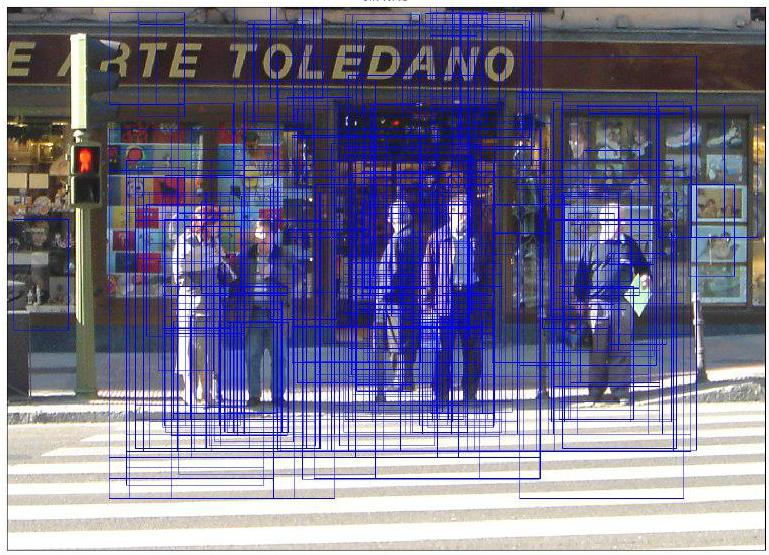
\includegraphics[width=.46\textwidth]{SinNMS-1.jpg}
						\end{varwidth}
					}
					\fbox{
						\begin{varwidth}{\textwidth}
							\centering
							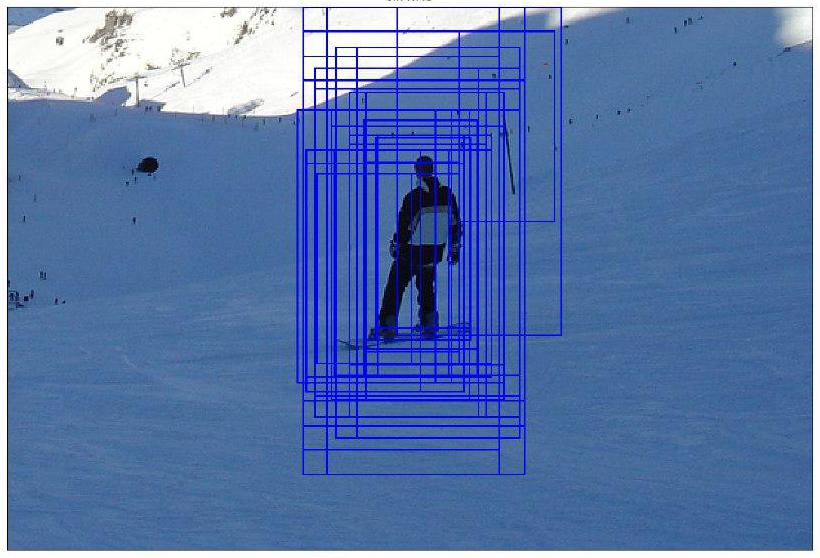
\includegraphics[width=.46\textwidth]{SinNMS-2.jpg}
						\end{varwidth}
					}
                    \fbox{
						\begin{varwidth}{\textwidth}
							\centering
							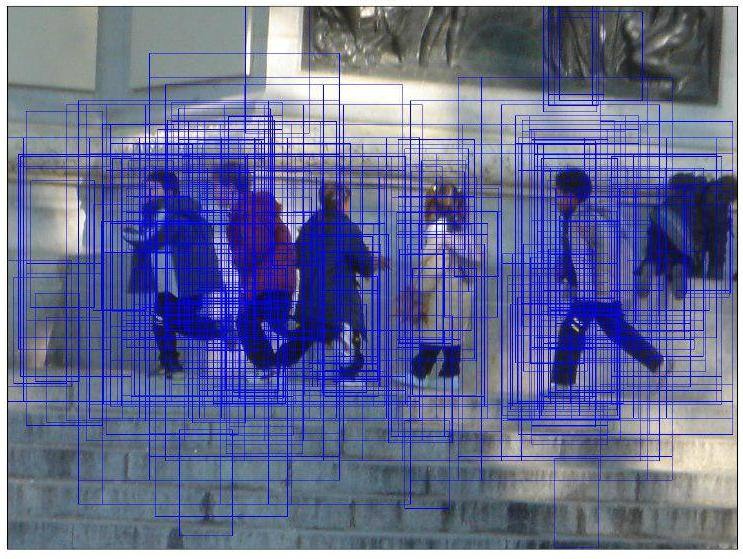
\includegraphics[width=.46\textwidth]{SinNMS-3.jpg}
						\end{varwidth}
					}
					\fbox{
						\begin{varwidth}{\textwidth}
							\centering
							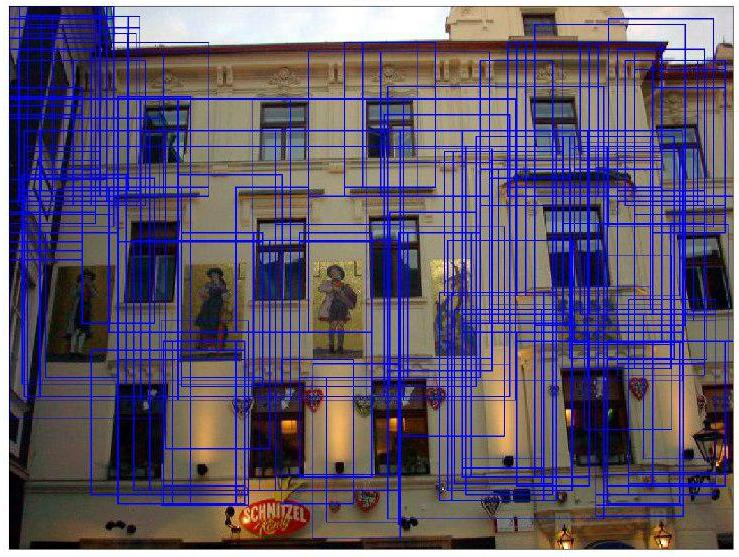
\includegraphics[width=.46\textwidth]{SinNMS-4.jpg}
						\end{varwidth}
					}

				\end{center}
				\caption{Positivos encontrados en 4 imágenes de muestra.}

			\end{figure}

            \par
            Se observa de forma clara que la tasa de error que obteníamos se convierte en un problema cuando evaluamos miles de ventanas por imagen. Por ello, es preciso tratar de dar soluciones.

            \subsubsection{Supresión de no máximos}

                \par
                Aunque no arreglará el problema de la calidad del modelo, una alternativa para descartar muchos de los falsos positivos es la supresión de no máximos (\textit{NMS}). La idea aquí es aprovechar el grado de confianza del clasificador en que una ventana contenga un peatón y descartar todas aquéllas que se solapen en cierta medida con una de mayor confianza. Veamos cómo hacer esto:

                \NMS[label=.]{../pedestrian_detection.py}

                \par
                Ya que para cada ventana positiva habíamos guardado las coordenadas de sus esquinas superior izquierda e inferior derecha junto con su confianza, lo primero que hacemos es separar los datos para mayor claridad. Seguidamente, las ordenamos de mayor a menor confianza (nótese que \texttt{I} es un vector de índices) y calculamos sus áreas.

                \par
                Ahora comienza el proceso de descarte. En cada iteración seleccionamos la ventana con mayor confianza de entre las que quedan sin procesar y calculamos la proporción de su solapamiento con las demás (dividiendo entre sus áreas). Se guarda la ventana en cuestión y se eliminan todas aquellas que se superpongan más de un cierto umbral (fijado aquí a 0.3 mediante experimentación).

                \par
                Como consecuencia de añadir la supresión de no máximos, el procedimiento de búsqueda se ve ligeramente alterado:

                \EscaneoNMS[label=.]{../pedestrian_detection.py}

                \par
                En la pregunta al clasificador hemos usado \texttt{decision\_function}, que devuelve la distancia al hiperplano separador, porque necesitamos medidas de confianza en las predicciones para utilizarlas en \texttt{non\_maximum\_suppression}. Si \texttt{decision\_function} da un valor mayor que 0, la muestra está en la clase positiva; si da menor que 0, está en la clase negativa.

                \par
                Como prueba del efecto que tiene la supresión de no máximos, comparemos los resultados anteriores con los obtenidos usando este filtro:

                \begin{figure}[H]

    		        \begin{center}

    		        	\setlength{\fboxrule}{0pt}
                        \fbox{
    						\begin{varwidth}{\textwidth}
    							\centering
    							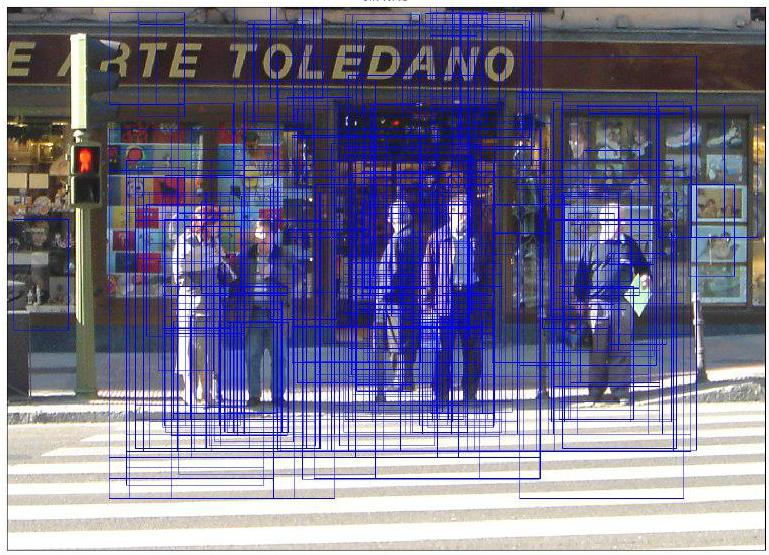
\includegraphics[width=.46\textwidth]{SinNMS-1.jpg}
    						\end{varwidth}
    					}
                        \fbox{
    						\begin{varwidth}{\textwidth}
    							\centering
    							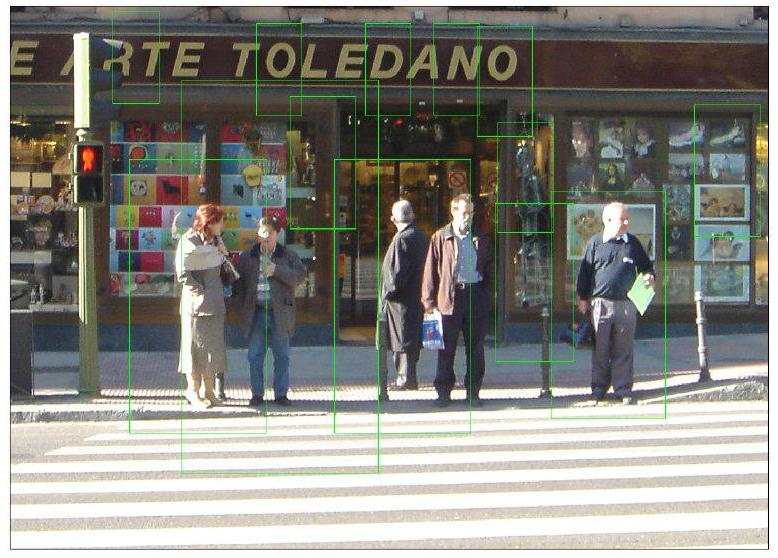
\includegraphics[width=.46\textwidth]{ConNMS-1.jpg}
    						\end{varwidth}
    					}
                        \fbox{
    						\begin{varwidth}{\textwidth}
    							\centering
    							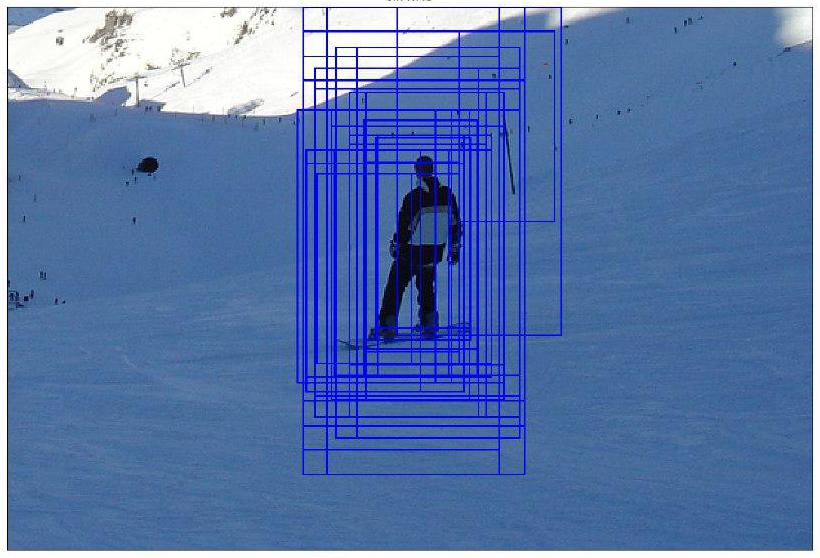
\includegraphics[width=.46\textwidth]{SinNMS-2.jpg}
    						\end{varwidth}
    					}
    					\fbox{
    						\begin{varwidth}{\textwidth}
    							\centering
    							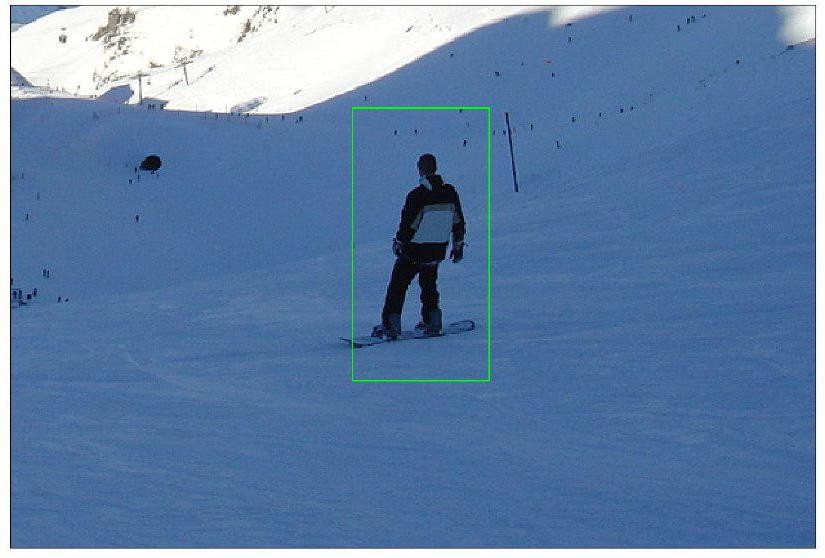
\includegraphics[width=.46\textwidth]{ConNMS-2.jpg}
    						\end{varwidth}
    					}
                        \fbox{
    						\begin{varwidth}{\textwidth}
    							\centering
    							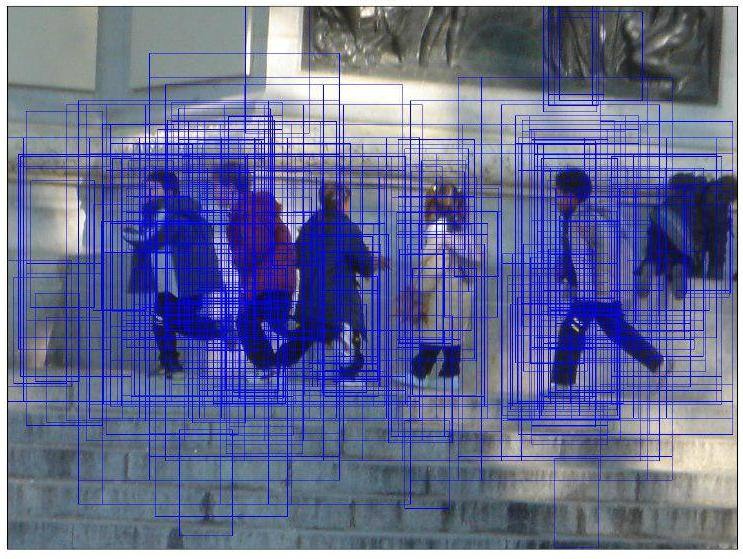
\includegraphics[width=.46\textwidth]{SinNMS-3.jpg}
    						\end{varwidth}
    					}
                        \fbox{
    						\begin{varwidth}{\textwidth}
    							\centering
    							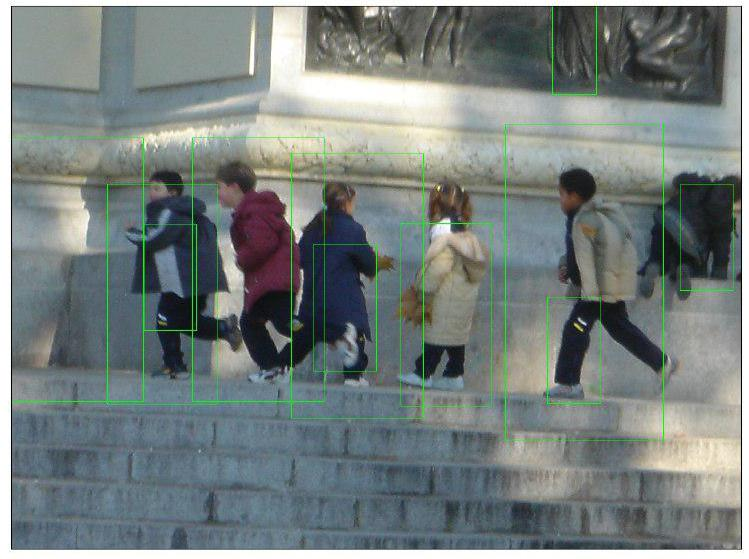
\includegraphics[width=.46\textwidth]{ConNMS-3.jpg}
    						\end{varwidth}
    					}
                        \fbox{
    						\begin{varwidth}{\textwidth}
    							\centering
    							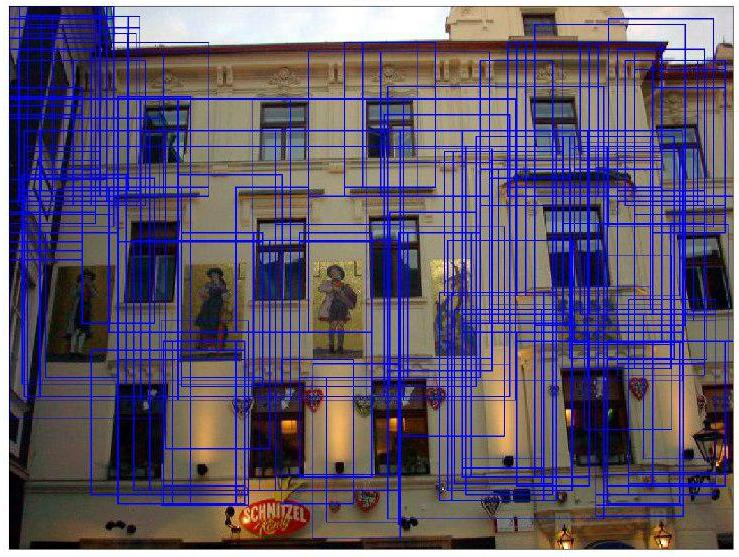
\includegraphics[width=.46\textwidth]{SinNMS-4.jpg}
    						\end{varwidth}
    					}
    					\fbox{
    						\begin{varwidth}{\textwidth}
    							\centering
    							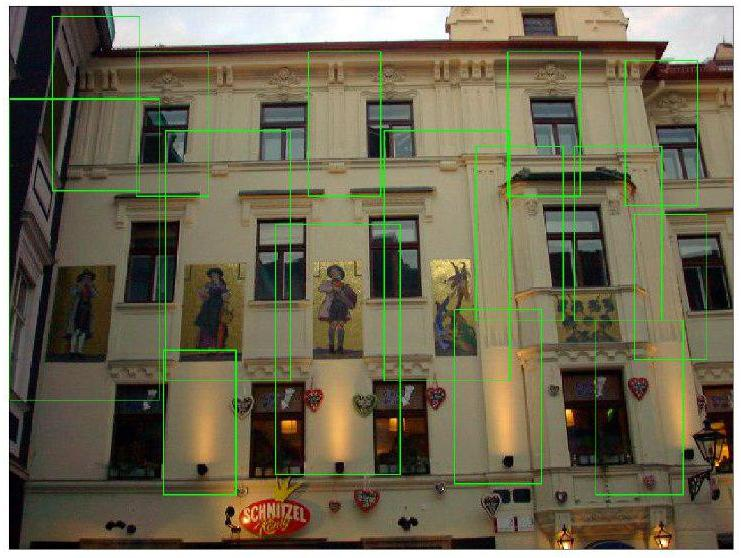
\includegraphics[width=.46\textwidth]{ConNMS-4.jpg}
    						\end{varwidth}
    					}

    				\end{center}
    				\caption{Comparación de positivos en las 4 imágenes de muestra con y sin supresión de no máximos.}

    			\end{figure}

                \par
                De lo anterior podemos concluir que la supresión de no máximos es de gran ayuda, pero que la utilidad del proceso que realiza depende del modelo. En nuestro caso, aún queda un número notable de imprecisiones.

                \par
                Para concluir el análisis de esta mejora, veamos la penalización en tiempo de ejecución, tanto considerando el proceso tal cual como añadiendo el posterior dibujado:

                \begin{table}[H]

    				\centering

    				\begin{tabular}{| >{\centering\arraybackslash}m{0.9in} | >{\centering\arraybackslash}m{1in} | >{\centering\arraybackslash}m{1in} | >{\centering\arraybackslash}m{1in} | >{\centering\arraybackslash}m{1in} |}

    					\hline
    					\textbf{Imagen} & \textbf{Tiempo original (s)} & \textbf{Tiempo \textit{NMS} (s)} & \textbf{Tiempo original + dibujado (s)} & \textbf{Tiempo \textit{NMS} + dibujado (s)}\\
    					\hline
    					Imagen 1 & 65.83891 & 66.18080 & 70.66711 & 70.39946 \\
    					\hline
    					Imagen 2 & 12.39770 & 12.29394 & 14.35838 & 13.94862 \\
    					\hline
    					Imagen 3 & 68.98459 & 70.52982 & 74.14415 & 73.80650 \\
    					\hline
                        Imagen 4 & 20.54199 & 20.53334 & 23.24827 & 22.88052 \\
                        \hline

    				\end{tabular}

    			\end{table}

                \par
                En la tabla se aprecia que la pérdida de velocidad es mínima, y que incluso obtenemos beneficio si abarcamos también la posterior fase de dibujado de las ventanas.

            \subsubsection{Selección por votación}

                \par
                Asumiendo el uso de \textit{NMS}, otra manera de intentar arreglar el problema es utilizar varios clasificadores y elegir la clase de una imagen por mayoría simple. Veamos cómo se han entrenado:

                \EntrenamientoClasificadores[label=.]{../pedestrian_detection.py}

                \par
                Recibiendo como parámetro los conjuntos completos de muestras, entrenamos cada uno de los $n$ clasificadores con todos los ejemplos positivos y con un subconjunto aleatorio de ejemplos negativos, de forma que las clases estén equilibradas.

                \par
                Para la decisión por mayoría simple, lo único que hemos de hacer es sumar los votos y dividir por el número de clasificadores; si supera 0.5, se acepta como positivo:

                \ClasificadorVotos[label=.]{../pedestrian_detection.py}

                \par
                Finalmente, la función actualizada queda de la siguiente manera:

                \EscaneoVotos[label=.]{../pedestrian_detection.py}

                \par
                Como vemos, el único cambio es que la clasificación ahora toma en cuenta el voto por mayoría, siendo afirmativo en caso de que su proporción supere el 50\%.

                \par
                Comparemos ahora los nuevos resultados con los obtenidos en la supresión de no máximos:

                \begin{figure}[H]

    		        \begin{center}

    		        	\setlength{\fboxrule}{0pt}
                        \fbox{
    						\begin{varwidth}{\textwidth}
    							\centering
    							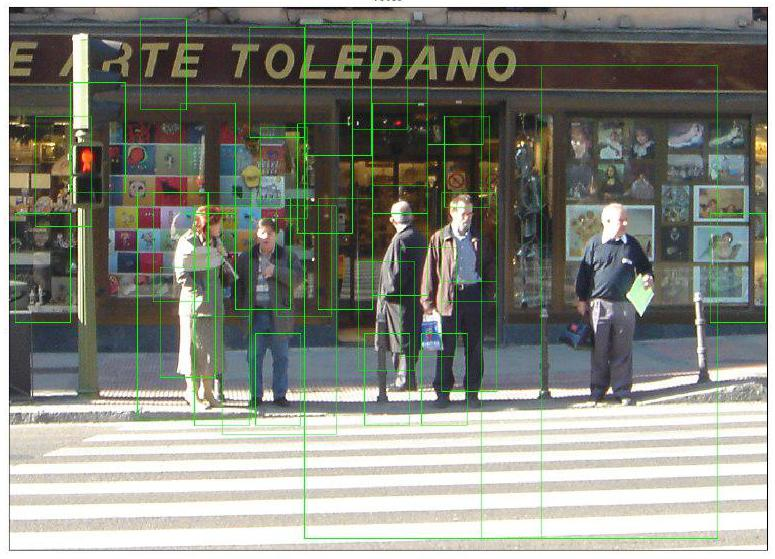
\includegraphics[width=.46\textwidth]{ConVotos-1.jpg}
    						\end{varwidth}
    					}
                        \fbox{
    						\begin{varwidth}{\textwidth}
    							\centering
    							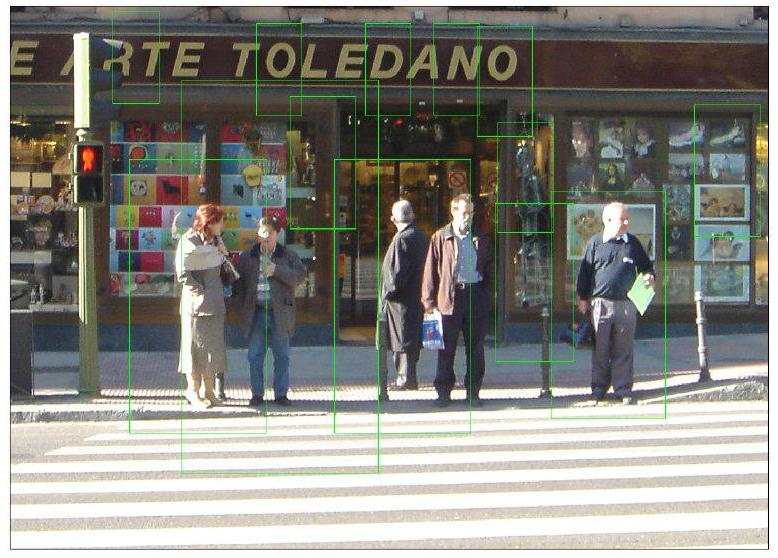
\includegraphics[width=.46\textwidth]{ConNMS-1.jpg}
    						\end{varwidth}
    					}
                        \fbox{
    						\begin{varwidth}{\textwidth}
    							\centering
    							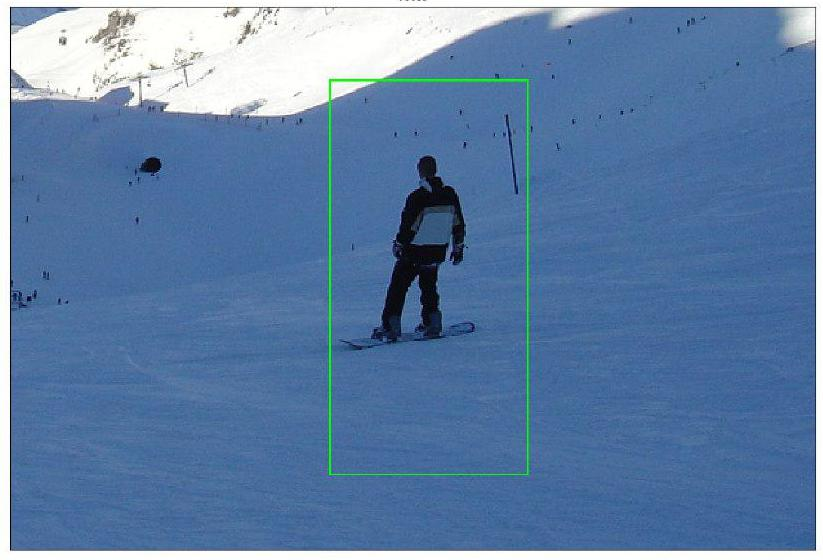
\includegraphics[width=.46\textwidth]{ConVotos-2.jpg}
    						\end{varwidth}
    					}
    					\fbox{
    						\begin{varwidth}{\textwidth}
    							\centering
    							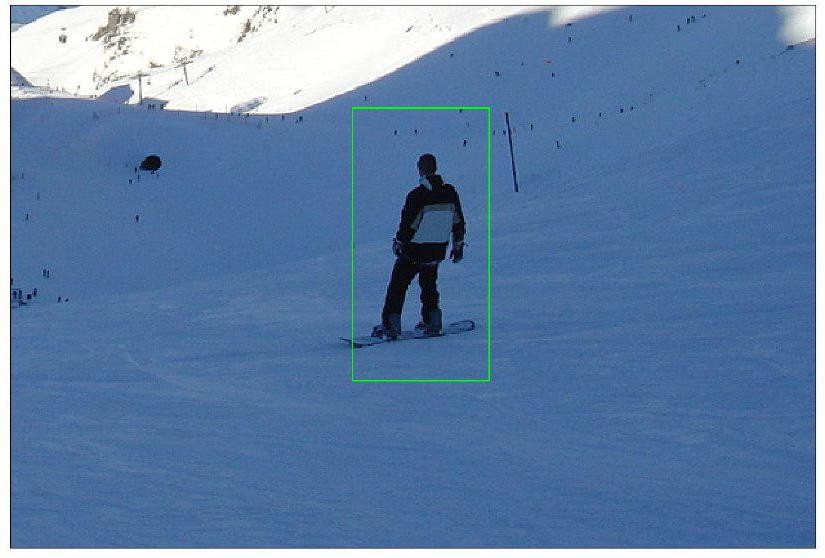
\includegraphics[width=.46\textwidth]{ConNMS-2.jpg}
    						\end{varwidth}
    					}
                        \fbox{
    						\begin{varwidth}{\textwidth}
    							\centering
    							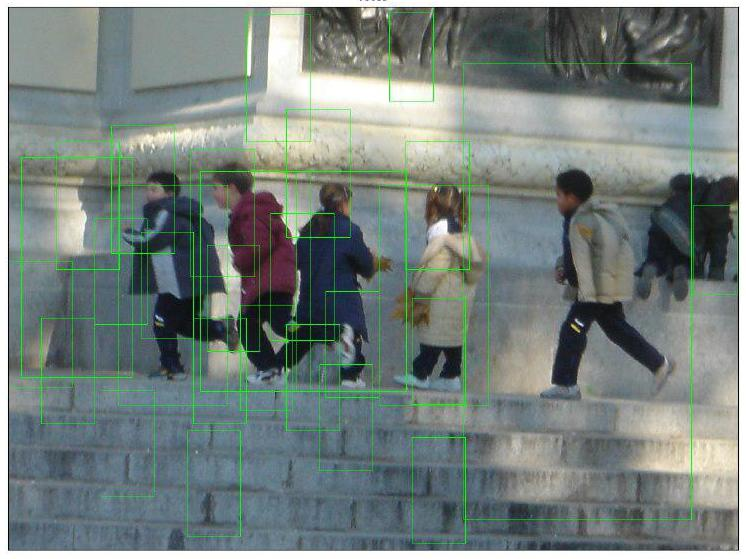
\includegraphics[width=.46\textwidth]{ConVotos-3.jpg}
    						\end{varwidth}
    					}
                        \fbox{
    						\begin{varwidth}{\textwidth}
    							\centering
    							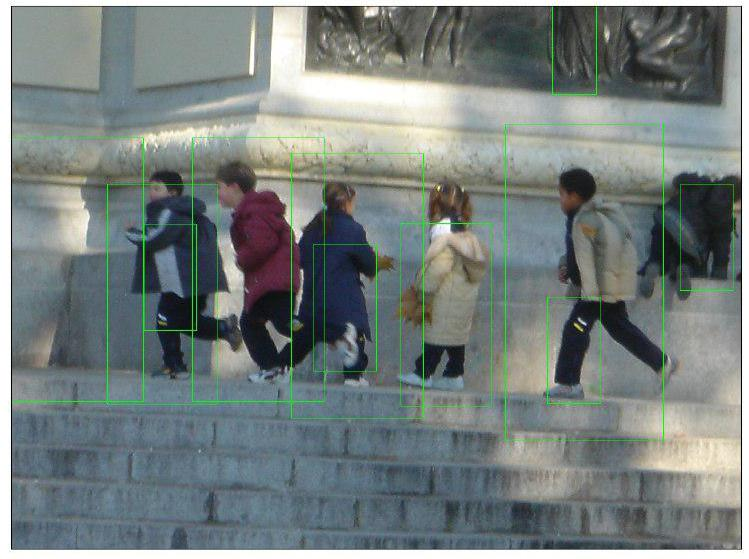
\includegraphics[width=.46\textwidth]{ConNMS-3.jpg}
    						\end{varwidth}
    					}
                        \fbox{
    						\begin{varwidth}{\textwidth}
    							\centering
    							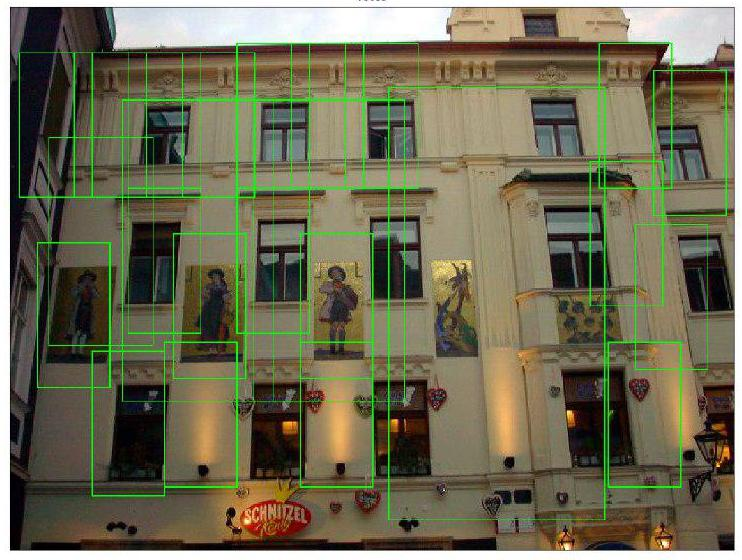
\includegraphics[width=.46\textwidth]{ConVotos-4.jpg}
    						\end{varwidth}
    					}
    					\fbox{
    						\begin{varwidth}{\textwidth}
    							\centering
    							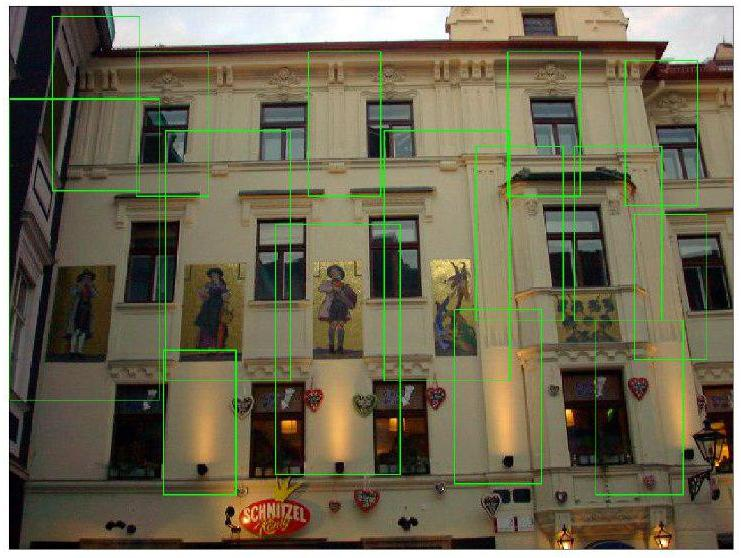
\includegraphics[width=.46\textwidth]{ConNMS-4.jpg}
    						\end{varwidth}
    					}

    				\end{center}
    				\caption{Comparación de resultados con votos (izquierda) y sin votos (derecha).}

    			\end{figure}

                \par
                El sistema de votos, probado con 11 \textit{SVM}s, parece dar peores resultados en cuanto a falsos positivos. Sin embargo, al final de la sección analizaremos todas las alternativas para sacar algunas conclusiones más.

            \subsubsection{Incrementando el umbral}

                \par
                Otra posibilidad para rebajar la tasa de falsos positivos es elevar el umbral a partir del cual consideramos que una imagen contiene un peatón. La desventaja de esto es que aumentará el número de falsos negativos, pero el equilibrio entre ambos tipos de errores es una cuestión que trataremos más adelante.

                \par
                La librería \texttt{scikit-learn} contiene varias formas de utilizar un modelo \textit{SVM}. La implementación más eficiente y escalable no ofrece la posibilidad de devolver la confianza (en tanto por 1) de la predicción, por lo que sólo podríamos usar la implementación más lenta, que sí tiene tal funcionalidad.

                \par
                Sin embargo, realizando pruebas obtenemos que una regresión logística tiene un acierto del 98.6\% en test, muy similar a nuestro mejor resultado.





\end{document}
